% !TEX root = MAIN.tex


\chapter{Code-driven Mutation Testing}
\label{chapter:codeDriven}

\section{General description}


\subsection{Product perspective}

\RQ{} The code-driven mutation testing component (in Chapter~\ref{chapter:codeDriven}, referred to as \emph{the system}) implements the Mutation Testing Process for code-driven mutation testing described in D2.

\RQ{} The code-driven mutation testing component is not released as a single executable file but consists of a set of executable programs.

\clearpage
\subsection{General capabilities}

\RQ{} The code-driven mutation testing component shall implement the process for the evaluation of test suite effectiveness that is drafted in Figure~\ref{fig:process:codeDriven:evaluation}. Figure~\ref{fig:process:codeDriven:evaluation} relies on UML activity diagram notation. In Figure~\ref{fig:process:codeDriven:evaluation} the execution of specific software artefacts from the end user is made explicit. Also, we use black arrows to draw control-flow, red arrows for data-flow. Each activity is described in Section~\ref{sec:rquirements:capabilities}.

\begin{figure}[h]
  \centering
	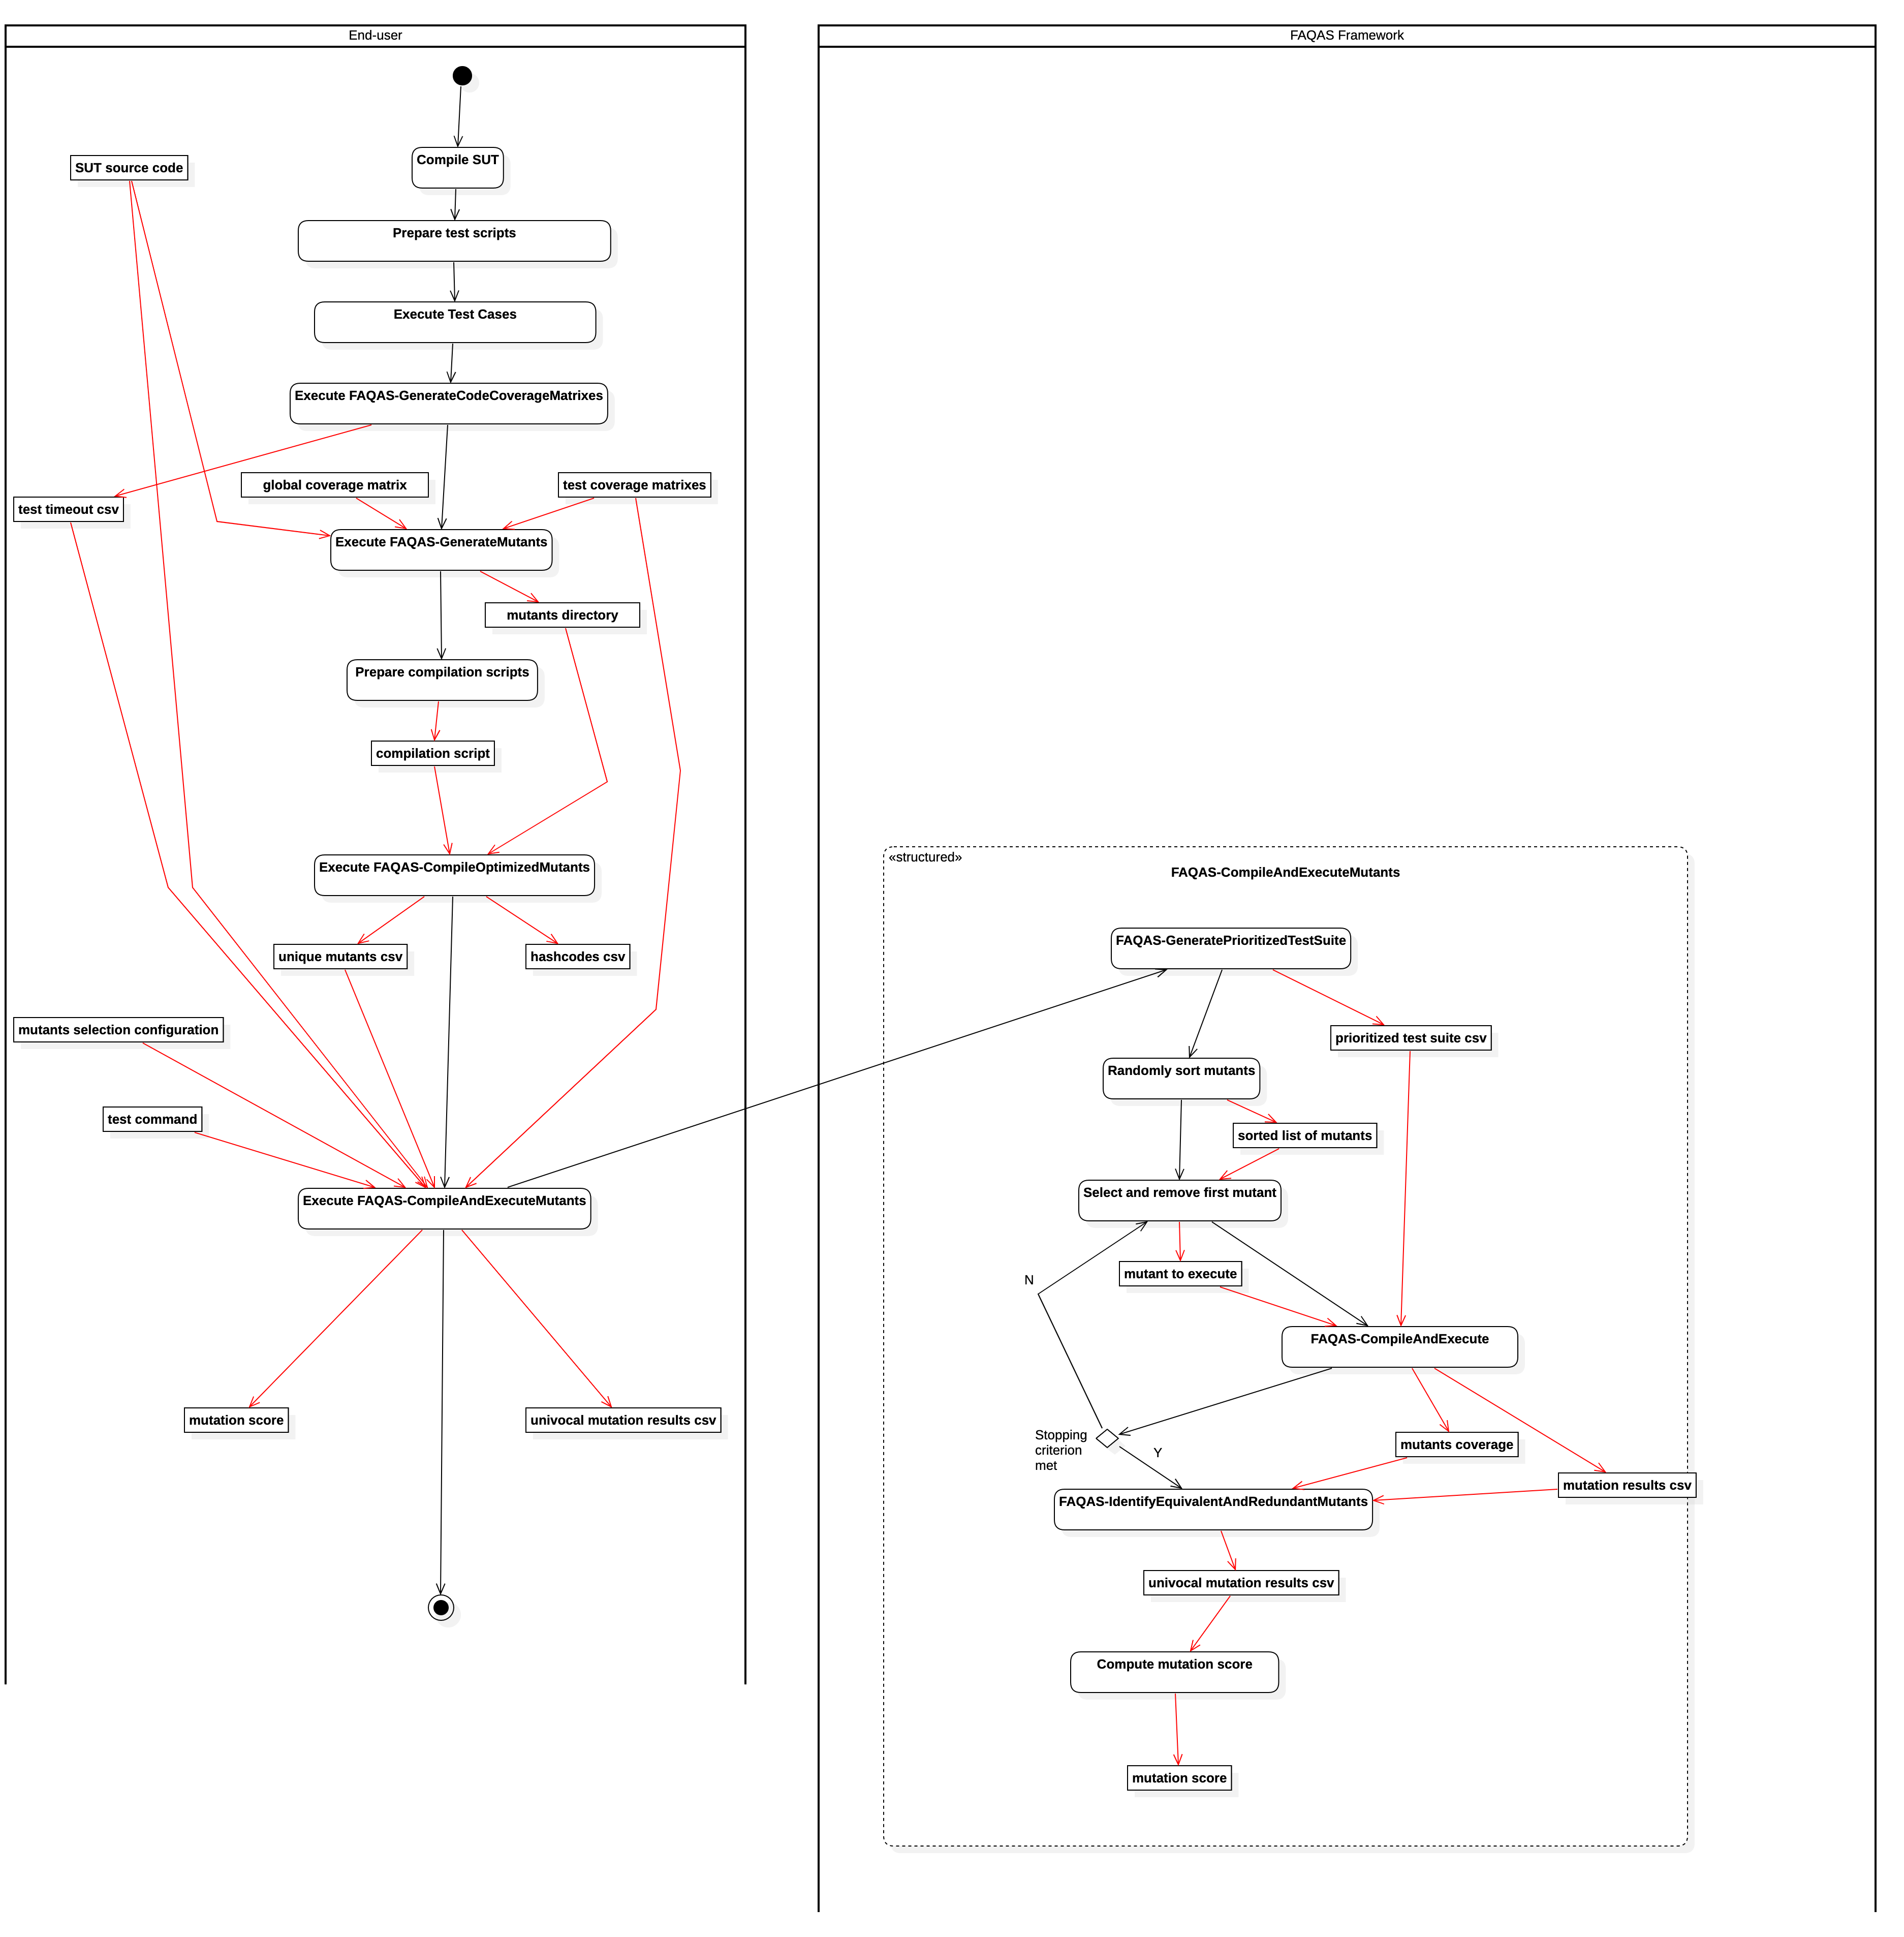
\includegraphics[width=15cm]{images/png/Activity1!CodeDrivenTestSuiteEvaluation_1.png}
      \caption{Overview of the code-driven mutation testing process to evaluate test suite effectiveness.}
      \label{fig:process:codeDriven:evaluation}
\end{figure}


\RQ{} The code-driven mutation testing component shall implement the process for the improvement of the effectiveness of test suites that is drafted in Figure~\ref{fig:process:codeDriven:augmentation}. Figure~\ref{fig:process:codeDriven:augmentation} relies on UML activity diagram notation. In Figure~\ref{fig:process:codeDriven:augmentation} the execution of specific software artefacts from the end user is made explicit. Also, we use black arrows to draw control-flow, red arrows for data-flow. Each activity is described in Section~\ref{sec:rquirements:capabilities}.

\begin{figure}[h]
  \centering
	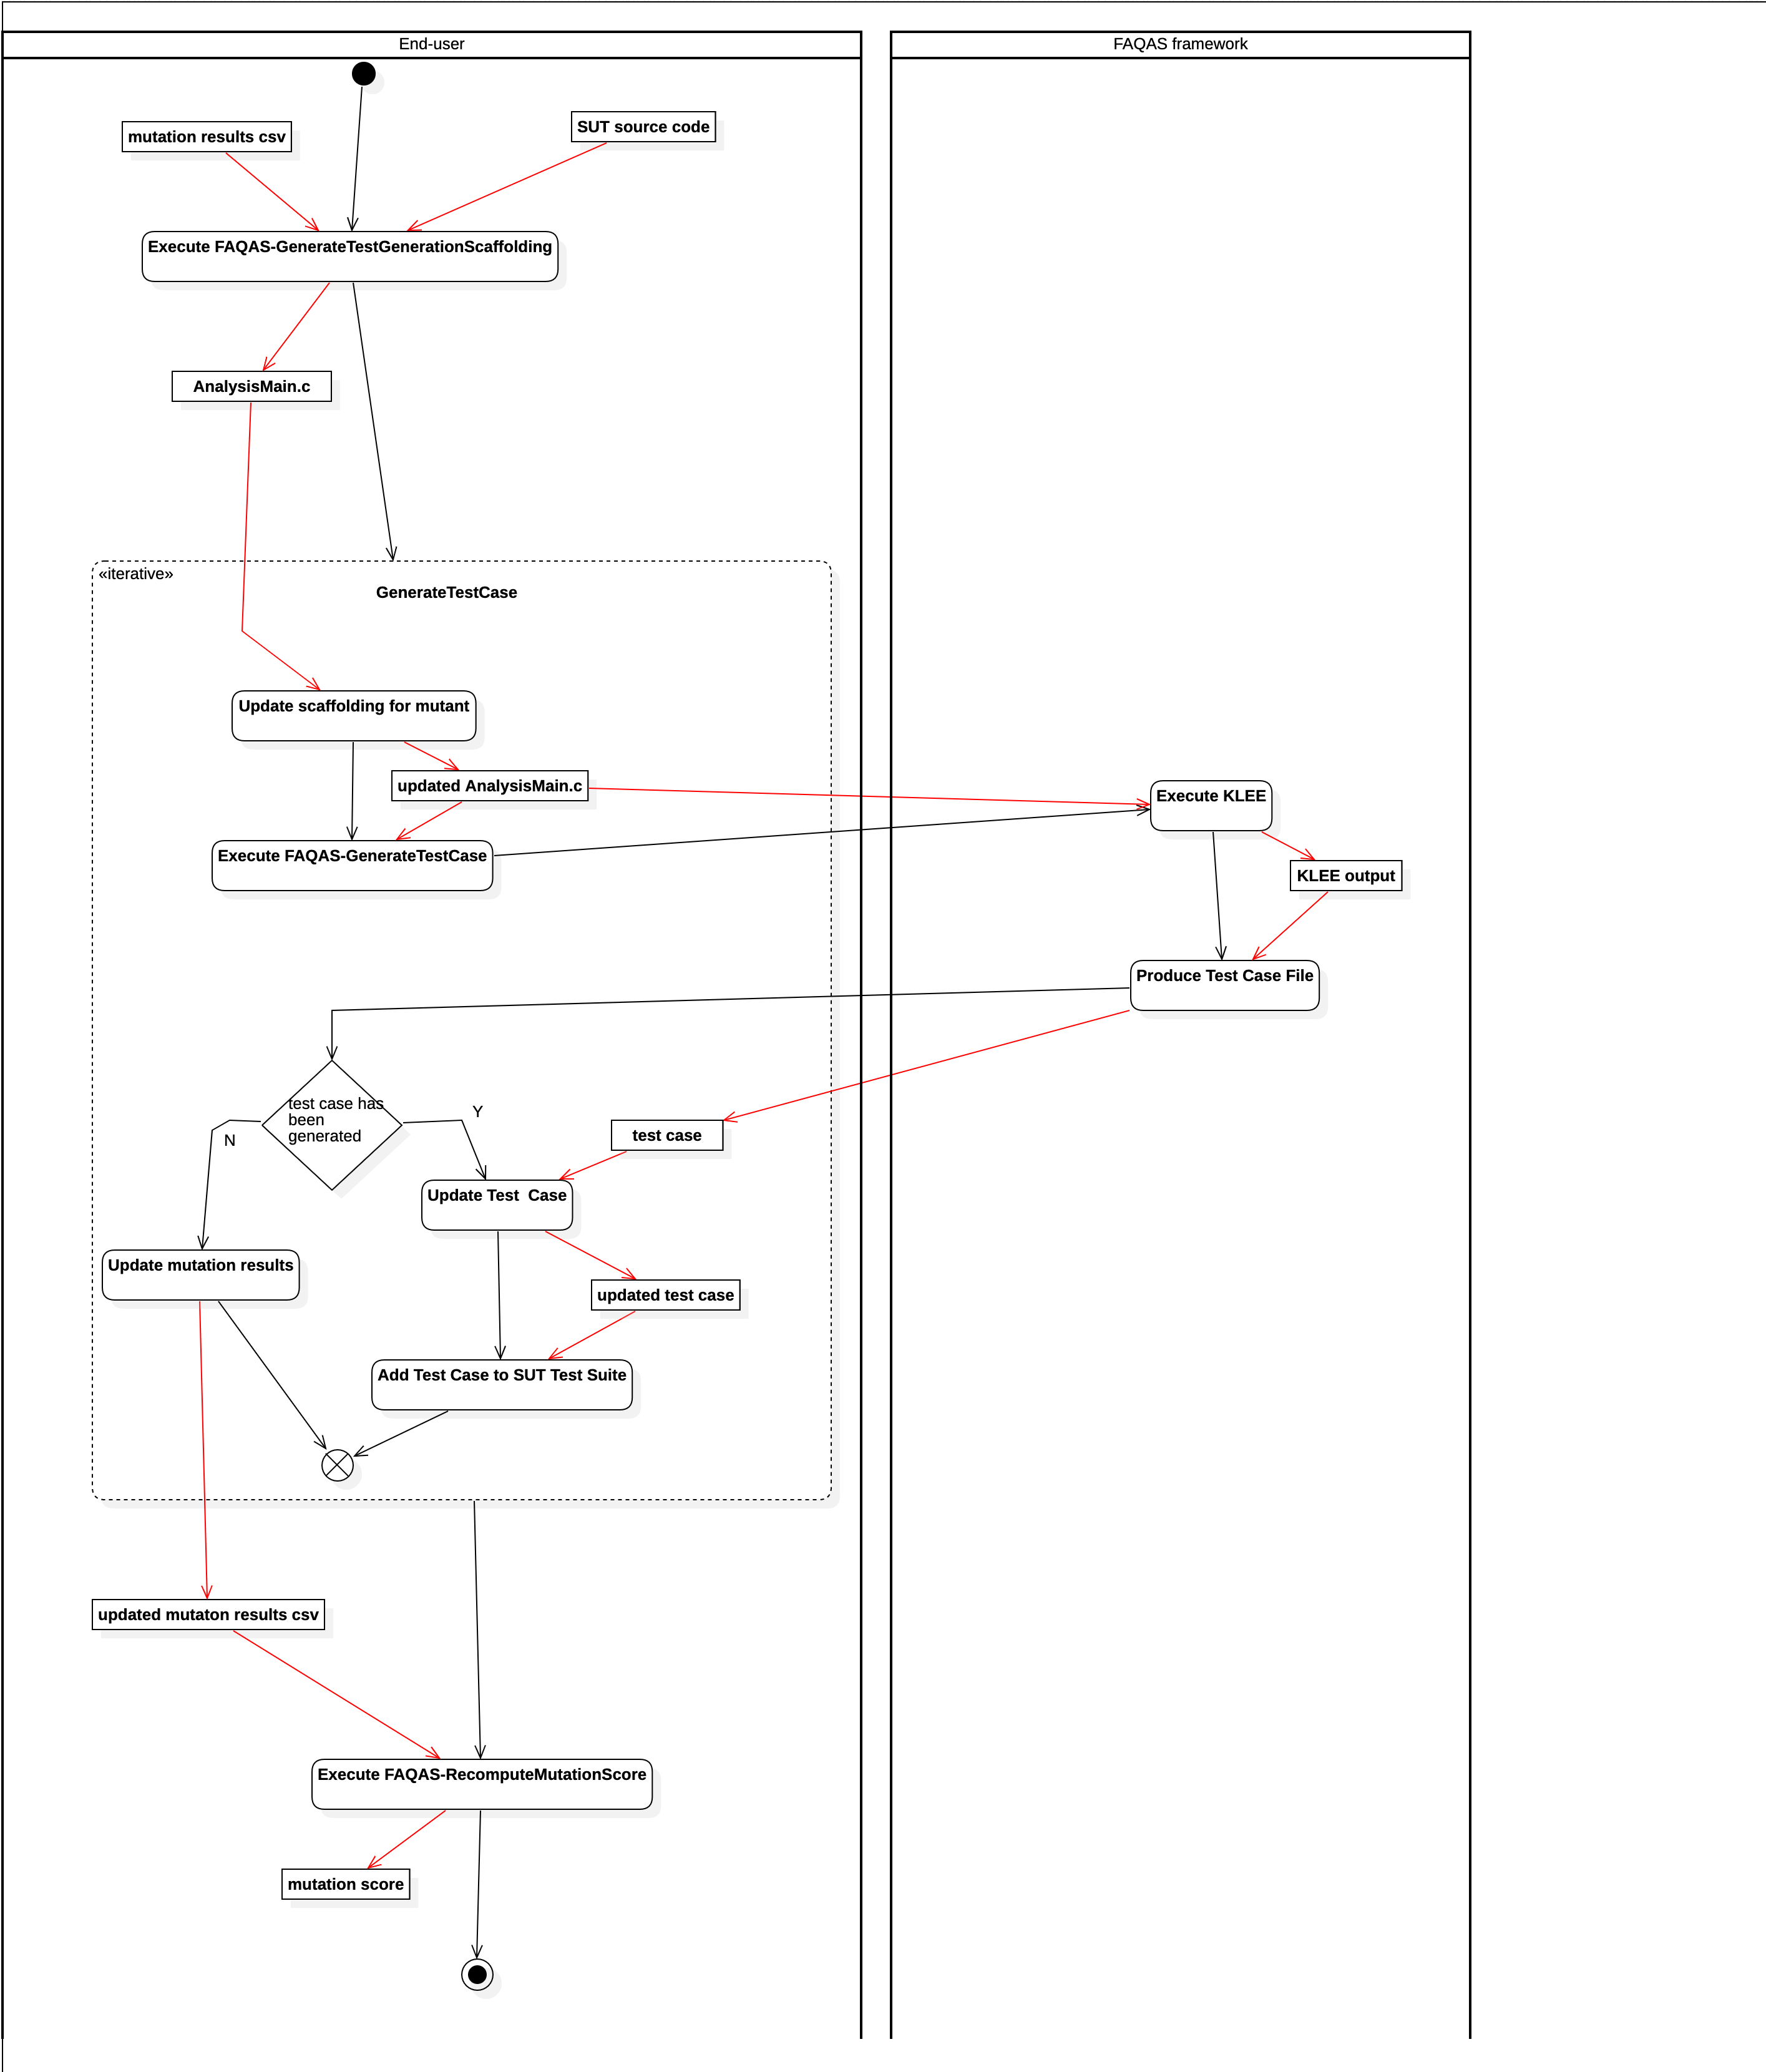
\includegraphics[width=15cm]{images/png/Activity1!CodeDrivenTestSuiteAugmentation_2.png}
      \caption{Overview of the code-driven test suite augmentation process.}
      \label{fig:process:codeDriven:augmentation}
\end{figure}


\clearpage

\subsection{General constraints}

\RQ{} The automated generation of test cases (i.e., the objective of test suite augmentation) is an open, complex, research problem. For this reason, it is necessary to rely on existing tools (see D2 for detailed discussion).

\RQ{} The automated generation of test cases shall rely on KLEE, which is the most stable test case generation tool, based on WP2 evaluation.

\clearpage

\subsection{Operational environment}

% cosi generale?
\RQ{} The system shall be executed on a Linux operating system with a Bash shell.



\subsection{Assumptions and dependencies}

\RQ{} The system targets SUT built using either GCC Make~\footnote{https://gcc.gnu.org/onlinedocs/gccint/Makefile.html} or WAF\footnote{https://waf.io/}.

\RQ{} The system mutates and generate test cases for SUT compiled with GCC~\footnote{https://gcc.gnu.org}.

\RQ{} The test suite of the SUT is implemented as a script (hereafter, \emph{test suite script}) either a Makefile or a Bash script. Each test case is executed through the invocation of a command in the script.

\section{Specific requirements}
%\section{General}
\subsection{Capabilities requirements}
\label{sec:rquirements:capabilities}

%\RQ{} The gcov coverage information associated to each test case shall be stored in a separate directory.

\RQ{} The activity \emph{Compile SUT} in Figure~\ref{fig:process:codeDriven:evaluation} indicates that the engineers shall compile  the SUT with coverage options enabled.

\RQ{} The activity \emph{Prepare test scripts} in Figure~\ref{fig:process:codeDriven:evaluation} concerns extending the \emph{test suite script} for the SUT to store the code coverage of each single test case separately. This is achieved by adding a call to a dedicated bash script provided by FAQAS (\emph{FAQAS-CollectCodeCoverage}) after the execution of every test case.

\RQ{} The activity \emph{Execute test cases} in Figure~\ref{fig:process:codeDriven:evaluation} concerns the execution of the test cases following the practice for the SUT (e.g., running the command \texttt{make test}).

\RQ{} The activity \emph{Execute FAQAS-GenerateCodeCoverageMatrix} in Figure~\ref{fig:process:codeDriven:evaluation} concerns the execution of a provided program delivered with the FAQAS framework.

\RQ{} The activity \emph{Execute FAQAS-GenerateCodeCoverageMatrix} in Figure~\ref{fig:process:codeDriven:evaluation} generates a set of files: 
\begin{itemize}
\item one csv file referred to as \emph{global coverage matrix}, which indicates, for every line of code of the SUT, the ID of the test cases that cover the line of code;
\item a number of files  referred to as \emph{test coverage matrix}, one for each test case of the SUT. Each file indicates, for every line of code of the SUT, the number of times it has been covered during a single execution of the test case;
\item one file specifying, for each test case, a timeout value after which we shall consider a test case as hanging. The timeout value is generated by the system by triplicating the time taken by a test case launched in activity \emph{Execute test cases}.
\end{itemize}



\RQ{} Activity \emph{Execute FAQAS-GenerateMutants} in Figure~\ref{fig:process:codeDriven:evaluation} concerns the execution of the program \emph{FAQAS-GenerateMutants}. 

\RQ{} The program \emph{FAQAS-GenerateMutants} automatically generates a number of copies of each source file. Each copy contains one mutant.

% per ora abbiamo solo testato SRCIRor con files .c, dobbiamo valutare se funziona correttamente anche per .cpp
\RQ{} \emph{FAQAS-GenerateMutants} mutates source files implemented with C and C++ programming languages.

\RQ{} \emph{FAQAS-GenerateMutants} generates mutants by applying a set of mutation operators that can be selected by the end-users.

\RQ{} \emph{FAQAS-GenerateMutants} implements the set of operators listed in Table~\ref{table:operators}

% !TEX root =  ../Main.tex

\newcommand{\op}{\mathit{op}}
\newcommand{\ArithmeticSet}{ \texttt{+}, \texttt{-}, \texttt{*}, \texttt{/}, \texttt{\%} }
\newcommand{\LogicalSet}{ \texttt{&&}, \texttt{||} }
\newcommand{\RelationalSet}{ \texttt{>}, \texttt{>=}, \texttt{<}, \texttt{<=}, \texttt{==}, \texttt{!=} }
\newcommand{\BitWiseSet}{ \texttt{\&}, \texttt{|}, \land }
\newcommand{\ShiftSet}{ \texttt{>>}, \texttt{<<} }


\begin{table}[h]
\caption{Implemented set of mutation operators.}
\label{table:operators} 
\centering
\scriptsize
\begin{tabular}{|@{}p{4mm}@{}|@{}p{2cm}@{\hspace{1pt}}|@{}p{11.1cm}@{}|}
\hline
&\textbf{Operator} & \textbf{Description$^{*}$} \\
\hline
\multirow{7}{*}{\rotatebox{90}{\emph{Sufficient Set}}}&ABS               & $\{(v, -v)\}$	\\
\cline{2-3}
&AOR               & $\{(\op_1, op_2) \,|\, \op_1, \op_2 \in \{ \ArithmeticSet \} \land \op_1 \neq \op_2 \} $       \\
&    			  & $\{(\op_1, \op_2) \,|\, \op_1, \op_2 \in \{\texttt{+=}, \texttt{-=}, \texttt{*=}, \texttt{/=}, \texttt{\%} \texttt{=}\} \land \op_1 \neq \op_2 \} $       \\
\cline{2-3}
&ICR               & $\{i, x) \,|\, x \in \{1, -1, 0, i + 1, i - 1, -i\}\}$           \\
\cline{2-3}
&LCR               & $\{(\op_1, \op_2) \,|\, \op_1, \op_2 \in \{ \texttt{\&\&}, || \} \land \op_1 \neq \op_2 \}$            \\
&				  & $\{(\op_1, \op_2) \,|\, \op_1, \op_2 \in \{ \texttt{\&=}, \texttt{|=}, \texttt{\&=}\} \land \op_1 \neq \op_2 \}$            \\
&				  & $\{(\op_1, \op_2) \,|\, \op_1, \op_2 \in \{ \texttt{\&}, \texttt{|}, \texttt{\&\&}\} \land \op_1 \neq \op_2 \}$            \\
\cline{2-3}
&ROR               & $\{(\op_1, \op_2) \,|\, \op_1, \op_2 \in \{ \RelationalSet \}\}$            \\
&				  & $\{ (e, !(e)) \,|\, e \in \{\texttt{if(e)}, \texttt{while(e)}\} \}$ \\
\cline{2-3}
&SDL               & $\{(s, \texttt{remove}(s))\}$            \\
\cline{2-3}
&UOI               & $\{ (v, \texttt{--}v), (v, v\texttt{--}), (v, \texttt{++}v), (v, v\texttt{++}) \}$            \\   
\hline
\hline
\multirow{5}{*}{\rotatebox{90}{\emph{OODL}}}&AOD               & $\{((t_1\,op\,t_2), t_1), ((t_1\,op\,t_2), t_2) \,|\, op \in \{ \ArithmeticSet \} $       \\ 
\cline{2-3}
&LOD               & $\{((t_1\,op\,t_2), t_1), ((t_1\,op\,t_2), t_2) \,|\, op \in \{  \} \}$       \\ 
\cline{2-3}
&ROD               & $\{((t_1\,op\,t_2), t_1), ((t_1\,op\,t_2), t_2) \,|\, op \in \{ \RelationalSet \} \}$       \\ 
\cline{2-3}
&BOD               & $\{((t_1\,op\,t_2), t_1), ((t_1\,op\,t_2), t_2) \,|\, op \in \{ \BitWiseSet \} \}$       \\ 
\cline{2-3}
&SOD               & $\{((t_1\,op\,t_2), t_1), ((t_1\,op\,t_2), t_2) \,|\, op \in \{ \ShiftSet \} \}$       \\ 
%\hline
%COR               & $\{(\op_1, \op_2) \,|\, \op_1, \op_2 \in \{ \texttt{\&\&}, \texttt{||}, \land \} \land \op_1 \neq \op_2 \}$            \\
\hline
\hline
\multirow{3}{*}{\rotatebox{90}{\emph{Other}}}&LVR			& $\{(l_1, l_2) \,|\, (l_1, l_2) \in \{(0,-1), (l_1,-l_1), (l_1, 0), (\mathit{true}, \mathit{false}), (\mathit{false}, \mathit{true})\}\}$\\
&&\\
&&\\
\hline
\end{tabular}

$^{*}$Each pair in parenthesis shows how a program element is modified by the mutation operator. Th eleft element of the pair is replaced with the right element. We follow standard syntax~\cite{kintis2018effective}. Program elements are literals ($l$), integer literals ($i$), boolean expressions ($e$), operators ($\op$), statements ($s$), variables ($v$), and terms ( $t_i$, which might be either variables or literals).
\end{table}


% quindi, non produrremo anche una lista coi nomi dei mutanti + la sua location?
\RQ{} \emph{FAQAS-GenerateMutants} generates as output a directory tree (\emph{mutants directory} in Figure~\ref{fig:process:codeDriven:evaluation}) that follows the structure of the source directory tree of the SUT. However, every source file is replaced by a folder; the folder has the same name of the file. The folder contains all the mutants generated for that file. Every mutant has a name that univocally identifies it. The mutant name results from the conjunction of the following information:
source file name, mutated function name, mutated line, mutation operator name, mutation operation, mutated “column” (i.e., char position from the beginning of the line).
In the following, we report the structure of the output directory generated for a program

\begin{verbatim}
./src/store/vmem/vmem_checksum_first.c
./src/log/telemetry_appender.c

./src-mutants/store/vmem/vmem_checksum_first.c/
vmem_checksum_first.mut.145.7_1_13.ROR.vmem_param_load.c
./src-mutants/log/telemetry_appender.c/
telemetry_appender.mut.116.3_1_18.ROR.gs_log_appender_telem_append_isr.c
\end{verbatim}





\RQ{} Activity \emph{Prepare compilation scripts} in Figure~\ref{fig:process:codeDriven:evaluation} concerns the modification of the main compilation script for the SUT (e.g., the \emph{Makefile}). The engineer is expected to perform the following manual activities:
\begin{itemize}
\item Remove debugging flags
\item Remove coverage flags
\item Add a placeholder for the compiler optimization option
\item Add a 'sort' command in the source dependency list to ensure that source files are always compiled in the same order
\end{itemize}



\RQ{} Activity \emph{Execute FAQAS-CompileOptimizedMutants} in Figure~\ref{fig:process:codeDriven:evaluation} concerns the execution of the program \emph{FAQAS-CompileOptimizedMutants}.

\RQ{} The program \emph{FAQAS-CompileOptimizedMutants} compiles every mutant multiple times, once for every compiler optimization option selected by the end-user. It implements the pseudocode in Figure~\ref{alg:CompileOptimizedMutants}.

\begin{figure}[h]
\begin{algorithmic}[1]

%\footnotesize
\scriptsize


\Require \emph{OPT}, the set of compiler optimization options specified by the end-user
\Require \emph{MutantsDir}, path of the directory tree containing the mutants
\Require \emph{SUTsources}, path of the folder containing the sources of the SUT
\Require \emph{CompilatonCommand}, the command to execute to compile the original software

\Ensure \emph{hashcodes csv}, a csv file containing for every mutant, for every option, the SHA512 hashcode of the generated executable

\Ensure \emph{unique mutants}, a csv file containing the list of unique mutants. Unique mutants are mutants that are not equivalent and not redundant. See D2 for details.
% (source inputs, follow-up inputs, output data).

\For {OPT in OPTS}
\For {Mutant in MutantsDir}
\State Compile \emph{Mutant} with program \emph{FAQAS-CompileAndExecute}
\State Generate a SHA512 hash of the generated executable
\State Put the generated SHA512 hash in the \emph{hashcodes csv} file
\EndFor
\EndFor

\State Process \emph{hashcodes csv} and identify the \emph{unique mutants}
\State Save the list of \emph{unique mutants} in the output file \emph{unique mutants csv} 

\end{algorithmic}
\caption{FAQAS-CompileOptimizedMutants: Algorithm for compiling mutants with multiple optimization options}
%\vspace{-0.2cm}
\label{alg:CompileOptimizedMutants}
\end{figure}




\RQ{} Activity \emph{Execute FAQAS-CompileAndExecuteMutants} in Figure~\ref{fig:process:codeDriven:evaluation} concerns the execution of the program \emph{FAQAS-CompileAndExecuteMutants}.

\RQ{} The program \emph{FAQAS-CompileAndExecuteMutants} iterates over three activities: \emph{FAQAS-GeneratePrioritizedTestSuite}, \emph{FAQAS-CompileAndExecute}, \emph{FAQAS-IdentifyEquivalentAndRedundantMutants}. Each activity is implemented by a dedicated executable program that is invoked automatically by \emph{FAQAS-CompileAndExecuteMutants} without user intervention.

\RQ{} The program \emph{FAQAS-CompileAndExecuteMutants} takes as inputs the \emph{mutants selection configuration}, the \emph{unique mutants csv}, the path of the \emph{SUT source folder}, the \emph{command to execute test cases}, and the \emph{path to the folder containing the test coverage matrixes}.

\RQ{} The program \emph{FAQAS-CompileAndExecuteMutants} implements the four mutants selection strategies described in D2: \emph{all mutants}, \emph{proportional uniform sampling}, \emph{proportional method-based sampling}, \emph{uniform fixed-size sampling}, and \emph{uniform FSCI sampling}.

\RQ{} The \emph{mutants selection configuration} consists of the mutants selection strategy and a configuration value that specifies the number of mutants to consider. The format of the value that specifies the number of mutants to consider depends on the strategy; the value may indicate the percentage of mutants to sample (for \emph{proportional uniform sampling}, \emph{proportional method-based sampling}), the number of mutants to sample (for \emph{uniform fixed-size sampling}), the size of the confidence interval (for \emph{uniform FSCI sampling}).

\RQ{} The program\emph{FAQAS-GeneratePrioritizedTestSuite} takes as input the test coverage matrices and generates a file that specifies, for every line of the SUT, the prioritized list of test cases to execute (\emph{prioritized test suite csv}). This file indicates the sequence of test cases that shall be executed when testing a mutant affecting a certain line.

\RQ{} The activity \emph{Randomly sort mutants} indicates that  \emph{FAQAS-CompileAndExecuteMutants} generates a randomly sorted list of mutants. The list contains the mutants in \emph{unique mutants csv}.
In the case of \emph{proportional method-based sampling}, the list contains a set of mutants selected by following the stratified sampling strategy.

\RQ{} The activity \emph{Select and remove first mutant} indicates that  \emph{FAQAS-CompileAndExecuteMutants} selects the first mutant in \emph{sorted list of mutants} and removes it from the list.

\RQ{} The program \emph{FAQAS-CompileAndExecute} compiles a mutant by running the makefile of the original program; then it executes the SUT test suite. It follows the algorithm in Figure~\ref{alg:compileAndExecute}.


\begin{figure}[h]
\begin{algorithmic}[1]
\scriptsize
\Require \emph{Mutant}, path of the mutant to compile
\Require \emph{SUTsources}, path of the folder containing the sources of the SUT
\Require \emph{CompilatonCommand}, the command to execute to compile the original software
\Require \emph{TestCommand}, the command to execute to execute a single test case
\Require \emph{TestCases}, the prioritized list of test cases for the line of the mutant
\Require \emph{TestTimeout}, the max execution time that can be taken by the test case
\Ensure \emph{Result} KILLED or LIVE, based on test execution result (i.e., all test cases pass or one test case fails)
\State put \emph{Mutant} in place of the file it has been derived (\emph{original file}), keep the original file in a safe place
\State execute  \emph{CompilatonCommand} inside \emph{SUTsources}
\For {TestCase in TestCases}
\State execute the \emph{TestCase} by running \emph{TestCommand} inside \emph{SUTsources}
% succede qualcosa strano quando scrivi "the"
\If {the \emph{TestCase} fails (i.e., \emph{TestCommand} terminates with an error code)}
\State set \emph{Result} as KILLED
\State break the for loop
\EndIf
\If {the \emph{TestTimeout} expires}
\State set \emph{Result} as KILLED
\State break the for loop
\EndIf
\EndFor
\State move code coverage information in a subfolder of \emph{mutants coverage dir}
\State restore the \emph{original file}
\end{algorithmic}
\caption{FAQAS-CompileAndExecute: Algorithm to compile and test mutants}
\label{alg:compileAndExecute}
\end{figure}

\RQ{} The program \emph{FAQAS-CompileAndExecute} collects the mutation results of every mutant in a file, i.e., \emph{mutation results csv}. It contains, for every mutant, the indication of the mutation result (KILLED/LIVE).

\RQ{} The program \emph{FAQAS-CompileAndExecute} compiles and executes mutants till a termination criterion is met. The termination criterion depends on the mutants selection strategy (see D2 for details):
\begin{itemize}
\item \emph{all mutants}: the list \emph{sorted list of mutants} is empty
\item \emph{proportional uniform sampling}: a number of mutants matching the selected percentage has been executed
\item \emph{proportional method-based sampling}: the list \emph{sorted list of mutants} is empty
\item \emph{uniform fixed-size sampling}: a number of mutants matching the selected value has been executed
\item \emph{uniform FSCI sampling}: the confidence interval computed from \emph{mutation results csv} is smaller than the length specified by the user.
\end{itemize}

\RQ{} The program \emph{FAQAS-IdentifyEquivalentAndRedundantMutants} relies on code coverage information stored in \emph{mutants coverage dir} to identify equivalent and redundant mutants using the distance criterion $D_C$ (see D2).

\RQ{} The program \emph{FAQAS-IdentifyEquivalentAndRedundantMutants} generates a copy of \emph{mutation results csv} (i.e., \emph{univocal mutation results csv}) where only mutants that are considered non-equivalent and non-redundant are reported.

\RQ{} The activity \emph{Compile mutation score} concerns the computation of the mutation score based on the mutation results reported in \emph{univocal mutation results csv}.

\RQ{} The activity \emph{Execute FAQAS-CompileAndExecuteMutants} in Figure~\ref{fig:process:codeDriven:augmentation} concerns the execution of the program \emph{FAQAS-GenerateTestGenerationScaffolding}.

\RQ{} The program \emph{FAQAS-GenerateTestGenerationScaffolding} takes as input the path of the \emph{SUT source code} and the file \emph{mutation results csv}. It generates a number of files named \emph{MutatantId\_AnalysisMain.c}, one for each live mutant, where MutantId is the ID of a mutant. The file \emph{MutatantId\_AnalysisMain.c} contains a main function that should be used for the analysis with KLEE. 

\RQ{} The content of file \emph{MutatantId\_AnalysisMain.c} should resemble \emph{Listing 1.7} and \emph{Listing 1.9} of D2, it should enable the analysis with KLEE. For example, it should import the source file with the original function targeted by the mutation and the source code of the mutated function. Also, it should contain the definition of all the variables used for the execution of KLEE and a tentative set of required assertions.

\RQ{} The activity \emph{Update scaffolding for mutant} in Figure~\ref{fig:process:codeDriven:augmentation} indicates that the engineer should modify the file  \emph{MutatantId\_AnalysisMain.c} if necessary. In particular, it might be necessary to refine the assertions produced by \emph{FAQAS-GenerateTestGenerationScaffolding}. More precisely, since assertions should concern output variables, it is necessary to verify that all the necessary output variables had been referred in assertion. Indeed, in C, with pointers and pointers to pointers, it is not possible to have a precise automated identification of output variables.

\RQ{} The activities in the expansion region \emph{generateTestCase} are repeated for every live mutant.

\RQ{} The activity \emph{Execute FAQAS-GenerateTestCase} in Figure~\ref{fig:process:codeDriven:augmentation} concerns the execution of the program \emph{FAQAS-GenerateTestCase}.

\RQ{} The program \emph{FAQAS-GenerateTestCase} generates a tentative unit test case (i.e., a source file in C) that kills the mutant. It executes the KLEE program and then produces a unit test case (i.e., a file with a main in C) after processing the KLEE output.

\RQ{} For test generation, the support for the programming language of the SUT depends on KLEE (it supports C, limited support for C++).

\RQ{} The test case generated by \emph{FAQAS-GenerateTestCase} contains an invocation of the function under test (i.e., the function targeted  by the mutation) along with assigned arguments and an assertion that verifies results. The values for the assigned arguments and the verification of results are derived from the output of KLEE.

\RQ{} If the program \emph{FAQAS-GenerateTestCase} successfully generates a test case, the engineer proceeds with inspecting it (activity \emph{Update Test  Case}), otherwise he can consider the mutant as equivalent (activity \emph{Update mutation results}).

\RQ{} The activity \emph{Update Test  Case} in Figure~\ref{fig:process:codeDriven:augmentation} is performed by the engineer. He may need to execute the generated test case to verify that KLEE has generated valid inputs (e.g., inputs that meet the program preconditions). Based on KLEE results, \emph{FAQAS-GenerateTestCase} also generates assertions that reflect the output observed by KLEE (e.g., \texttt{assert( output == value\_observed\_by\_KLEE)} ). The engineer should thus also verify that the assertion with the expected value is correct (i.e., it reflects what indicated in the SUT specifications). If the value appearing in the assertion is not correct, it means that KLEE during its execution has observed an incorrect value being generated by the SUT; for this reason, the SUT might be faulty and should be fixed.

\RQ{} The activity \emph{Add Test Case to SUT Test Suite} in Figure~\ref{fig:process:codeDriven:augmentation} is performed by the engineer, who may add the new test case to the test suite.

\RQ{} The activity \emph{Update mutation results} in Figure~\ref{fig:process:codeDriven:augmentation} is performed when a test case is not generated. This generally happens when the mutant cannot be killed (i.e., is equivalent). The engineer is expected to manually inspect the mutant to be sure that the mutant is equivalent (otherwise the missing test case is due to a limitation of KLEE). If the mutant is equivalent the engineer removes it from the file \emph{mutation results csv}.

\RQ{} The activity \emph{Execute FAQAS-RecomputeMutationScore} in Figure~\ref{fig:process:codeDriven:augmentation}  concerns the execution of the program \emph{FAQAS-RecomputeMutationScore}. It is performed after generating test cases for all the live mutants. Program \emph{FAQAS-RecomputeMutationScore} recomputes the mutation score after ignoring the equivalent mutants detected by KLEE.

\subsection{System interface requirements}

\RQ{} The main user interface for the system is the command line.

\subsection{Adaptation and missionization requirements }

\RQ{} The system shall not be used in mission. The system is tool aimed at supporting the development of flight software. The system shall be used only to support development, validation, and verification activities in the development environment. 

\subsection{Computer resource requirements}

\RQ{} The system should be executed on a Linux operating system.

\subsection{Security requirements }

\RQ{} The system should not use network connections.

\subsection{Safety requirements}

\RQ{} To avoid safety hazards, the system shall not be used to assess test cases that are executed with target hardware in the loop.

\RQ{} The system cannot foresee the effect of mutation. If executed on the target hardware, the generated mutants might damage the target hardware or cause injuries to surrounding people.

\subsection{Reliability and availability requirements}

\RQ{} The system is expected to work according to is functional specifications every time it is invoked.

\RQ{} Since mutation testing execution time depends on both the number of mutants to be executed and the duration of the test suite execution, it is not possible to provide an upper bound for mutation testing execution time.

\subsection{Quality requirements}

\RQ{} Usability. Software engineers (i.e., professionals with a master degree in informatics or related fields) should be able to successfully use the software after reading its documentation.

\RQ{} Reusability. The software shall be used in any environment matching the characteristics indicated in this document.

\RQ{} Software development standards. The software development process shall follow ECSS guidelines as per SoW.

\subsection{Design requirements and constraints}

\RQ{} The system should be released with ESA Software Community Licence Permissive – v2.3”, as defined at https://essr.esa.int/. Any reused component should be compatible with the abovementioned licence.

\RQ{} The system shall be implemented using the bash shell script language, the Python programming language, and the C programming language.

\RQ{} The system shall mutate the source code of the SUT not the intermediate representation.

\subsection{Software operations requirements}

\RQ{} It should be possible to execute the system anytime, in an environment matching the characteristics indicated in this document.

\subsection{Software maintenance requirements}

\RQ{} One year maintenance support shall be provided as per SoW.

\subsection{System and software observability requirements}

\RQ{} To enable post-mortem debugging, all the temporary files generated by the system should be kept.

\section{Verification, validation and system integration}
 \subsection{Verification and validation process requirements}
 
 \RQ{} Every mutation operator should be tested by a dedicated unit test.
 
 \RQ{} A system test suite for the whole software should be provided. It should be based on the MLFS case study (see D2).
 
   \RQ{} The system should enable the correct  computation of the mutation score for the FAQAS case study systems indicated in deliverable D2.
 
 \subsection{Validation approach}

\RQ{} SnT is expected to perform a preliminary validation of the delivered framework.

 \RQ{} FAQAS industry partners are expected to use the system at their premises to validate it.
 

%  
% \subsection{Validation requirements}
% 
%
% 
% \subsection{Verification requirements}
% 
% \RQ{}

% \section{System models}
% 
% None reported.

